\begin{figure}[H]\centering
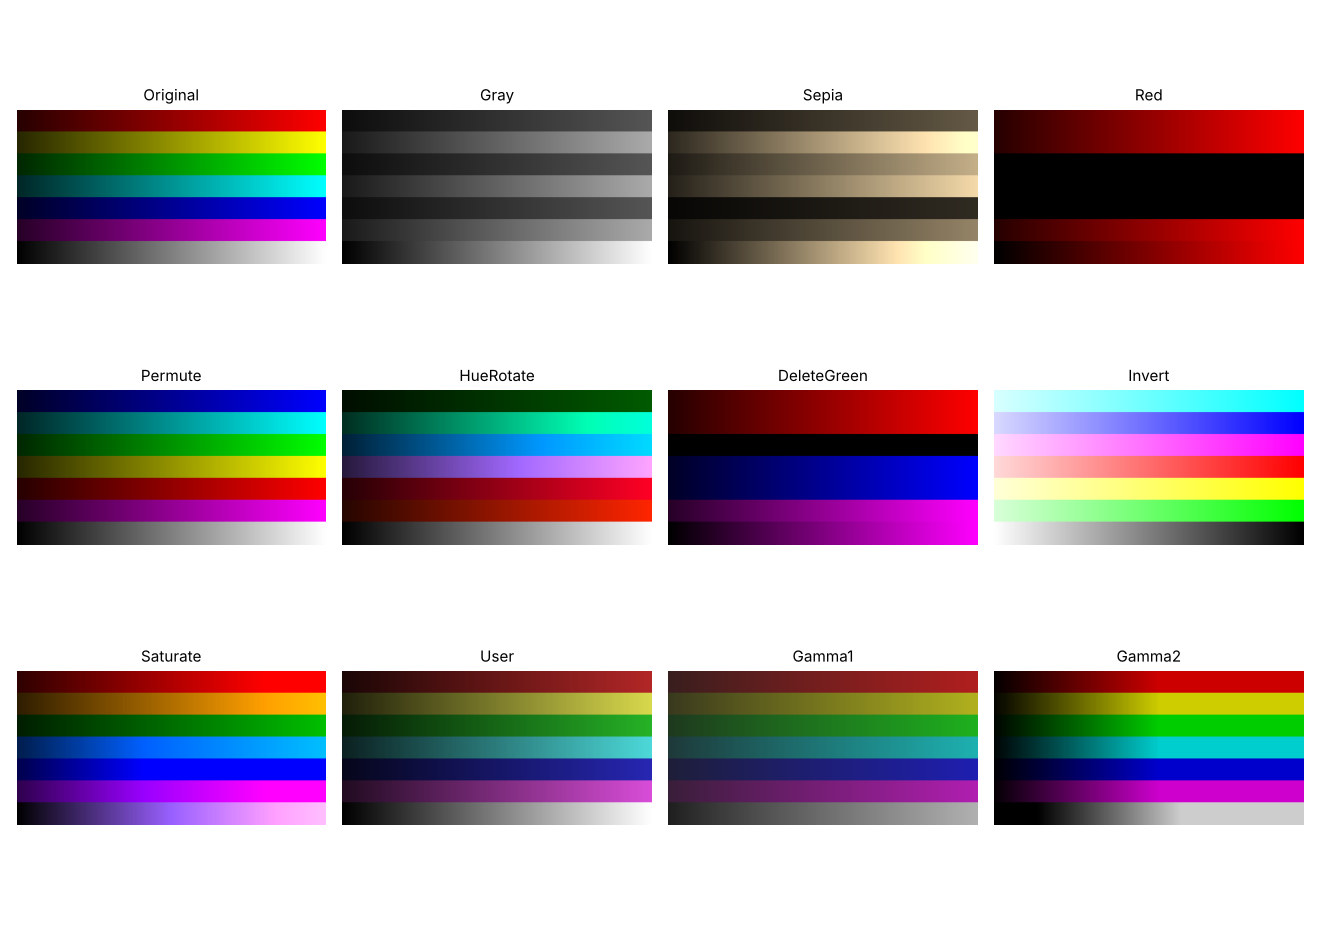
\includegraphics[width=\textwidth]{figures/luoi_bang_mau.png}
\caption{All filters applied to \texttt{bang\_mau}.}\label{fig:grid-bang_mau}
\end{figure}
\begin{figure}[H]\centering
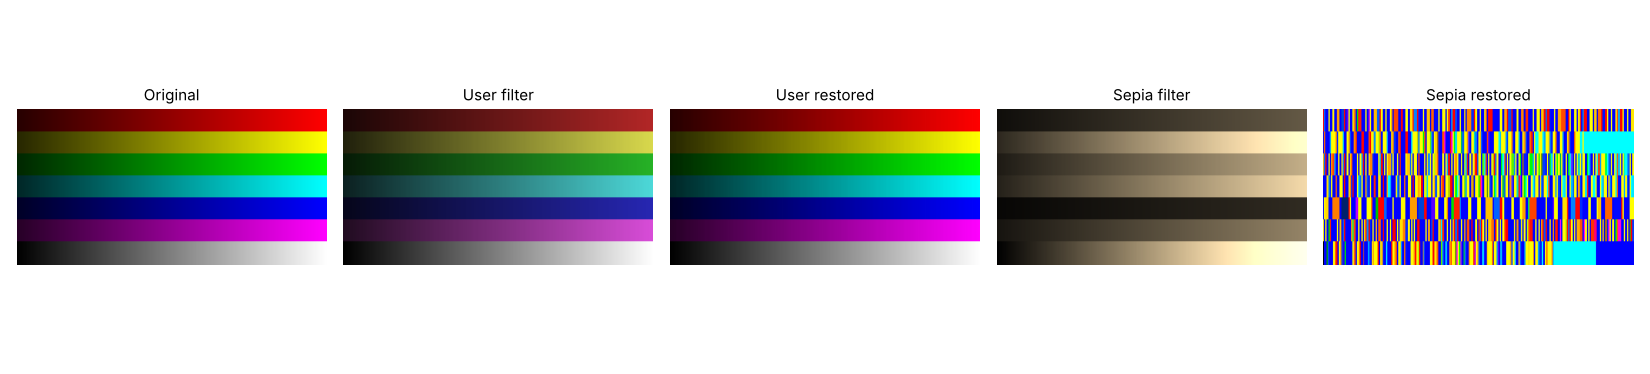
\includegraphics[width=\textwidth]{figures/khoi_phuc_bang_mau.png}
\caption{Inverse experiment on \texttt{bang\_mau}.}\label{fig:restore-bang_mau}
\end{figure}

\begin{figure}[H]\centering
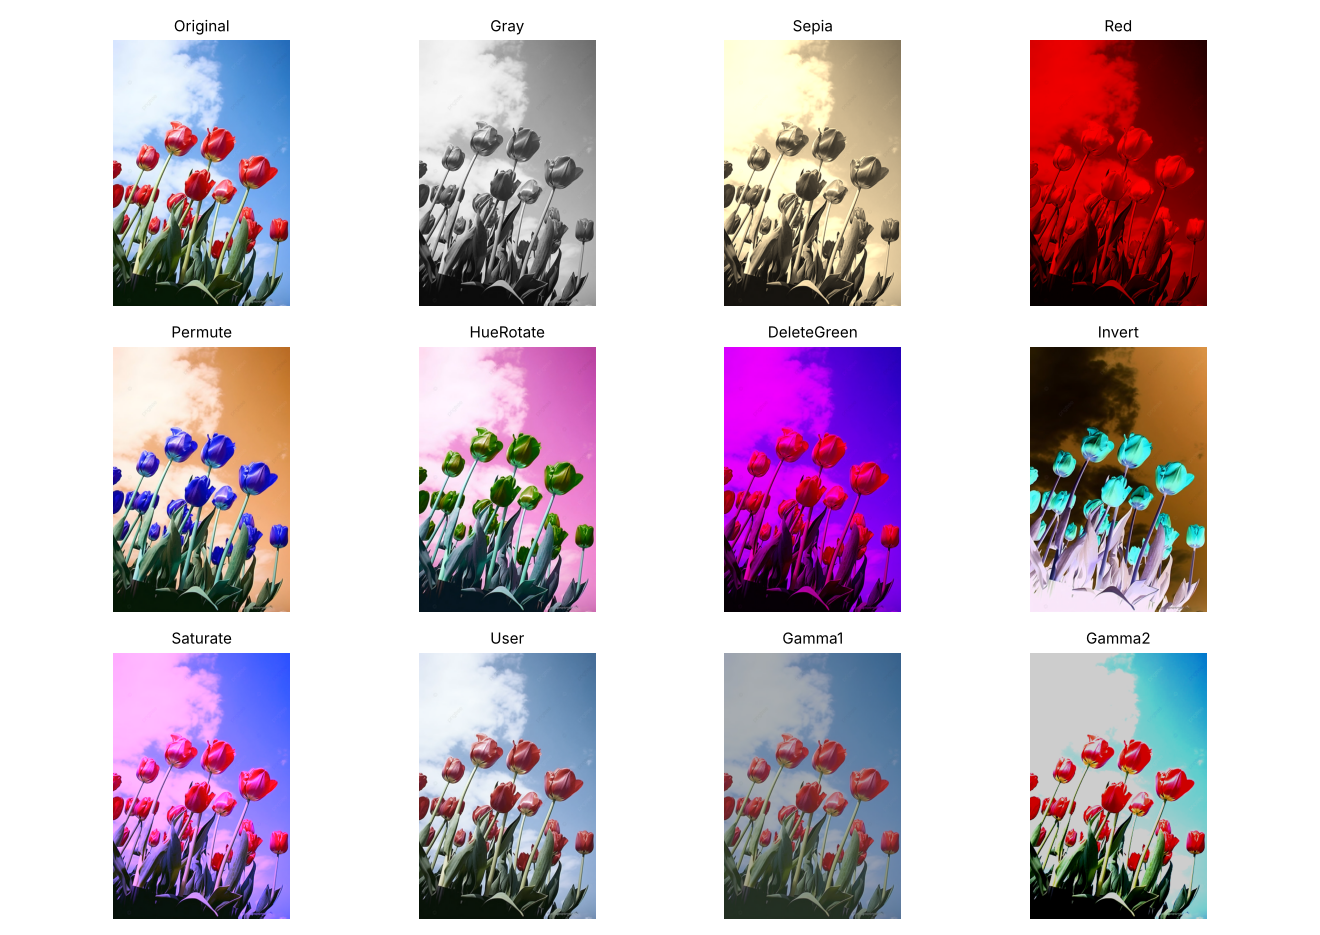
\includegraphics[width=\textwidth]{figures/luoi_TV6_anh1.png}
\caption{All filters applied to \texttt{TV6\_anh1}.}\label{fig:grid-TV6_anh1}
\end{figure}
\begin{figure}[H]\centering
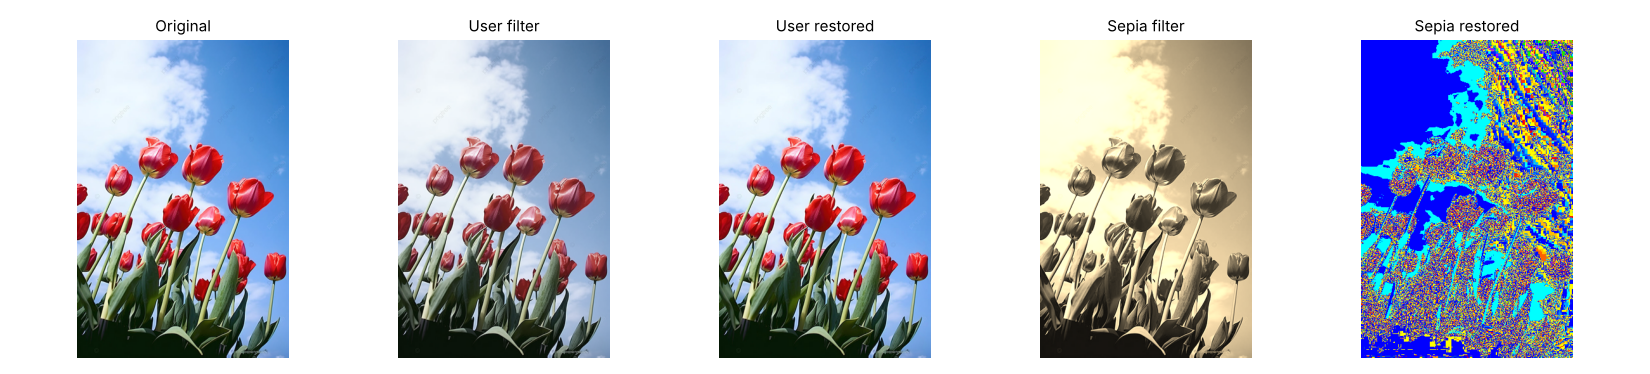
\includegraphics[width=\textwidth]{figures/khoi_phuc_TV6_anh1.png}
\caption{Inverse experiment on \texttt{TV6\_anh1}.}\label{fig:restore-TV6_anh1}
\end{figure}

\begin{figure}[H]\centering
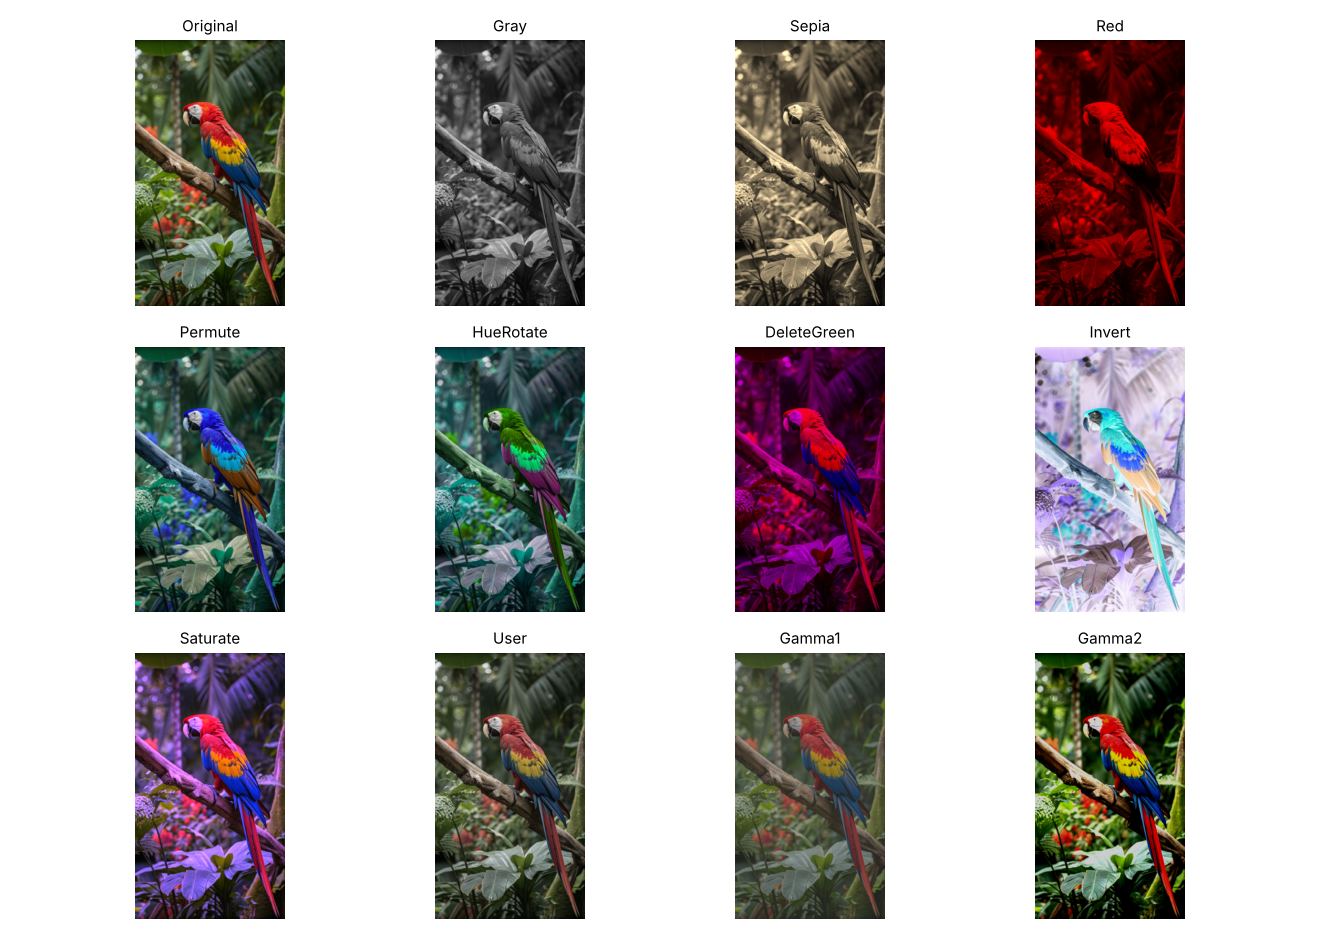
\includegraphics[width=\textwidth]{figures/luoi_TV6_anh2.png}
\caption{All filters applied to \texttt{TV6\_anh2}.}\label{fig:grid-TV6_anh2}
\end{figure}
\begin{figure}[H]\centering
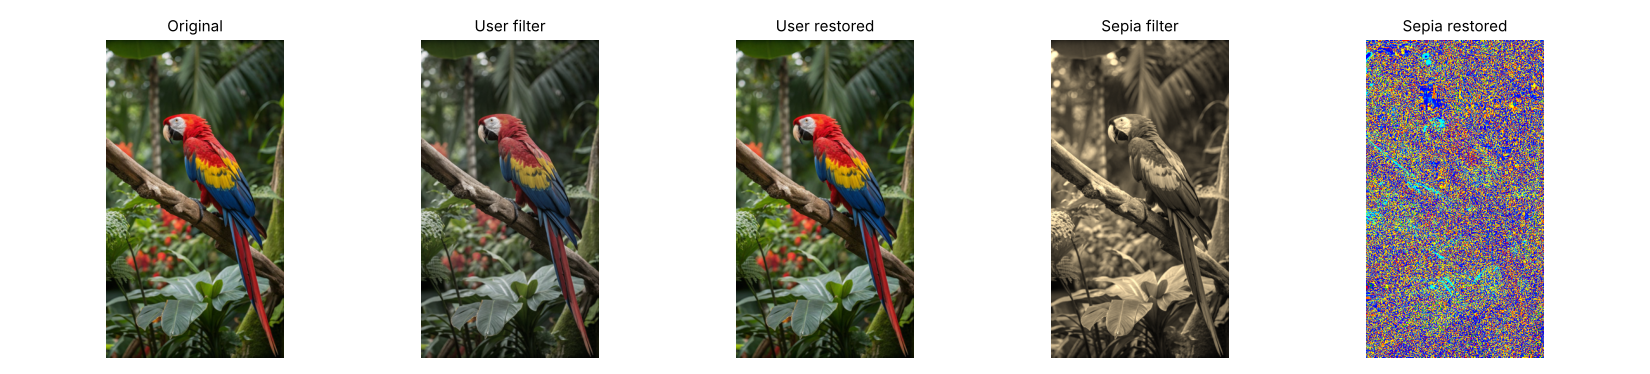
\includegraphics[width=\textwidth]{figures/khoi_phuc_TV6_anh2.png}
\caption{Inverse experiment on \texttt{TV6\_anh2}.}\label{fig:restore-TV6_anh2}
\end{figure}

\begin{figure}[H]\centering
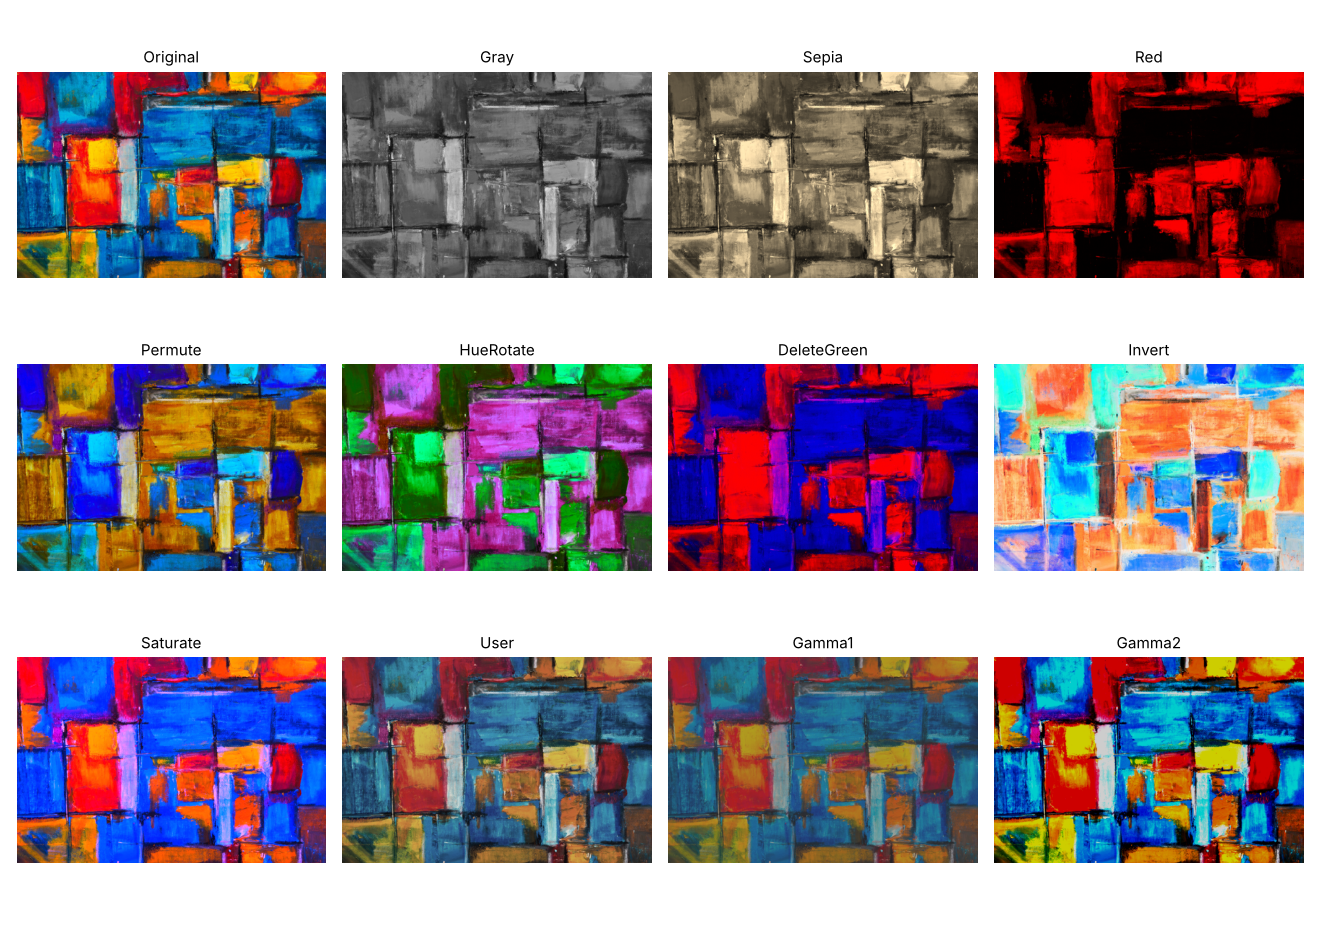
\includegraphics[width=\textwidth]{figures/luoi_TV6_anh3.png}
\caption{All filters applied to \texttt{TV6\_anh3}.}\label{fig:grid-TV6_anh3}
\end{figure}
\begin{figure}[H]\centering
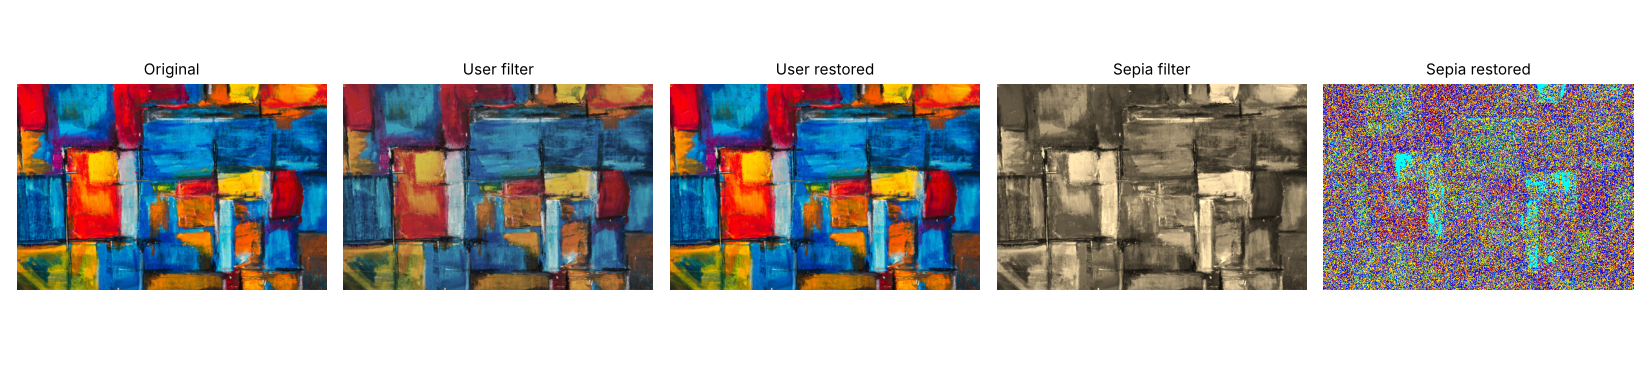
\includegraphics[width=\textwidth]{figures/khoi_phuc_TV6_anh3.png}
\caption{Inverse experiment on \texttt{TV6\_anh3}.}\label{fig:restore-TV6_anh3}
\end{figure}
